\documentclass[letterpaper,12pt]{article}
\usepackage[utf8]{inputenc}
\usepackage{fullpage}
\usepackage{courier}
\usepackage[margin=0.75in]{geometry}
\usepackage{listings}
\usepackage{color}
\usepackage{graphicx}
\usepackage[width=5in]{caption}
\usepackage{hyphenat}
\usepackage{hyperref}
\usepackage{float}
\usepackage{multirow}

% Format a sectionless paragraph
\newcommand*\unparagraph{
	\par
	\nopagebreak
	\vskip3.25ex plus1ex minus.2ex
	\noindent
}

% define extra colors
\definecolor{dkgreen}{rgb}{0,0.6,0}
\definecolor{purple}{RGB}{159,0,197}

% define the code listing format
\lstset{
	language=C++,
	basicstyle=\footnotesize\ttfamily,
	backgroundcolor=\color{white},
	showspaces=false,
	showstringspaces=false,
	frame=none,
	tabsize=3,
	keywordstyle=\color{purple},
	commentstyle=\color{dkgreen},
	stringstyle=\color{blue},
	escapeinside={\%*}{*)}
}

% efine the title/header
\title{\Large CS 3468\\Lab 5} 
\author{Jared Wallace}
\date{}

\begin{document}

\maketitle

\vspace{30mm}

\section*{Objectives}
\begin{enumerate}
\item Understand I/O control in a high level language
\item Understand the behavior of interrupts in a high level language
\end{enumerate}

\section*{Tasks}
\subsection*{Part 1: The reset interrupt}
The RESET interrupt is the entrance to a sensor application. When the reset button is pressed
(or the power is turned on), the RESET pin (PIN 20) of the ATmega128 processor triggers the 
RESET interrupt. The interrupt will initialize the sensor before giving control of the sensor
to the application.

An application written in a high level programming language does not directly control the action
of the RESET interrupt. Instead, the sensor's operating system provides a mechanism for the
application to initialize itself before it actually runs. In nesC, the RESET interrupt uses
the MainC component to initialize the sensor before subsequently firing the \emph{booted} event through
the \emph{Boot} interface to the application. Hence, in nesC, the application can make a routine in the
\emph{booted} event to be called each time the RESET interrupt is invoked.

Your job now is to make a routine such that each time the RESET button is pressed, an internal counter
of the application is incremented. Use the three LEDs to show the value of the current count.
(Hint: the RESET interrupt does not clear data memory unless being specified otherwise.)

Fill out the table below to indicate the mapping between the counter and the LED's:

\begin{table}[H]
\begin{center}
    \begin{tabular}{|c|c|c|c|}
        \hline
        \textbf{LED 0} & \textbf{LED 1} & \textbf{LED 2} & \textbf{Count} \\ \hline
         & & & 0 \\ \hline
         & & & 1 \\ \hline
         & & & 2 \\ \hline
         & & & 3 \\ \hline
         & & & 4 \\ \hline
         & & & 5 \\ \hline
         & & & 6 \\ \hline
         & & & 7 \\ \hline
    \end{tabular}
\end{center}
\end{table}

\subsection*{Part 2: UART communication in sensors}
UART is a type of serial communication between a sensor and another piece of equipment.
In our case, the sensor will send information to the computer through UART communication.
Accordingly, the sensor is the sender, and the computer will be the receiver. I will show
you how to receive data from the sensor via a handy dandy Java program.
The physical connection between your board and the computer will be via USB.

In nesC, the way you code for UART communication is very similar to the radio communication
we have already done. A sensor can send data via its USB port with the following two components:
SerialAMReceiverC (as receiver) and SerialActiveMessageC (as packet). The usage of the two
components is mostly same as the radio communication components AMReceiverC and ActiveMessageC.
The only differences are that (a) the “Serial.h” must be included, and (b) the destination address
(i.e., the computer) is 0.

To complete this section, you only need make a routine to send the internal count from the previous
section to the computer.

\section*{Lab Report}
\begin{enumerate}
   \item Please demonstrate your program to the lab instructor and let him check your code at the end of the current lab project.
   \item Your project report is due at the beginning of the next lab.
   \item Grading criteria
      \begin{itemize}
         \item Demonstration, 15 percent
         \item Code, 15 percent
         \item Report, 70 percent
      \end{itemize}
\end{enumerate}
\section*{Report instructions}
Format:
\begin{enumerate}
   \item Include your name and ID in the first page
   \item Font size of at least 10pt
   \item Single spaced
   \item Maximum of 5 pages (I will take points off for exceeding this without any good reason)
   \item Please submit as PDF online, and turn in a hard copy
\end{enumerate}
Content:
\begin{enumerate}
   \item Introduction (10 percent of your grade) Please summarize the task of this lab and what you have learned in the lab
   \item Reset interrupt (20 percent of your grade) Please describe in detail how you designed
       and implemented part one. Make a diagram (you can draw this by hand and attach it) of the
       components you used and how they are wired. Make sure you include how you implemented the counter.
    \item UART (40 percent of your grade) Please describe in detail how you designed and implemented part
        two. Attach a diagram (as before, this may be hand drawn) showing the components you used and
        how they are wired. Show me the result of the command:
        \begin{lstlisting}
        java -jar serial.jar hdlc
        \end{lstlisting}
        Discuss what layers in the OSI model these results belong to, and what (if any) data is in the other layers of the OSI model.
\end{enumerate}

% Comic at the bottom
\begin{figure}[ht!]
	\centering
	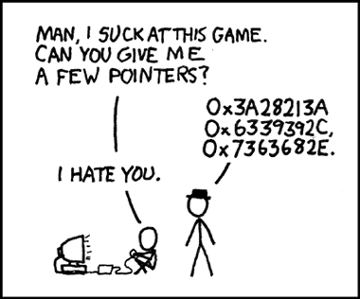
\includegraphics[width=4in]{pointers.png}
    \caption*{Every computer, at the unreachable memory address 0x-1, stores a secret.  I found it, and it is that all humans ar-- SEGMENTATION FAULT.}
\end{figure}

\end{document}
